\clearpage
\section{Autonomous Vehicles and Robots}

Autonomous robots or vehicles can work for an extended period of time gathering information from its surroundings to be able to work without human interaction. The robot or vehicle gathers different kinds of data, depending on what the goal of the device is. Positional data can be utilized for navigation and path finding in a known and unknown environment. Intelligent autonomous robots and vehicles are able to adapt to changes happening in its surroundings.
Currently there are many robots on the market that are self-reliant, ranging from autonomous vacuum cleaner to drones and helicopters. \cite{autonomousbasic}

Simple autonomous robots use ultrasonic sensors or infrared LEDS to manipulate its own behaviour if it detects obstacles or unexpected scenarios in the environment. This is useful for obstacle avoidance and mapping of unknown areas, where the robot through different reference points can pin-point the obstacles it has encountered along the way and in the future more efficiently avoid them.
More advanced robots use vision to grant them the ability to see their surroundings, algorithms analyse the vision data and gives the robot a depth perception, which grants the ability to instantly identify objects and locate them and memorize them immediately.\cite{obstacles}

There are two main kinds of autonomous robots, a single computer autonomous robot and insect robots. The single computer autonomous robot uses its own on-board computing unit to do its computations and its decisions, whereas the the insect robots are a fleet of many robots who are controlled by a single and separate computing unit.
The advantage of having a single computer autonomous robot is that the tasks it performs can be done using more dedicated computer resources. It has the possibility of utilizing the computing power to its full potential, instead of relying on a separate unit that is also making decisions and calculations for many other robots.
The insect robots are usually fairly simple in terms of capabilities, but the whole robot fleet can be utilized to perform advanced and possibly more sophisticated tasks, that requires a fleet simpler robots designed to work together autonomously.\cite{singleandinsect}


\clearpage
\section{Pathfinding and Mapping}

Pathfinding is done by a computer, where it uses plotting to find the shortest path between two different points. It can be viewed as an efficient way of navigating a maze. The main objective is getting from some location to a goal location.
There exists different pathfinding algorithms that are used for software simulations, but also for mobile robot navigation. Common pathfinding algorithms are A* (pronounced A star) and its extended version named D* (Dynamic A*).

\begin{figure}[H]
\centering
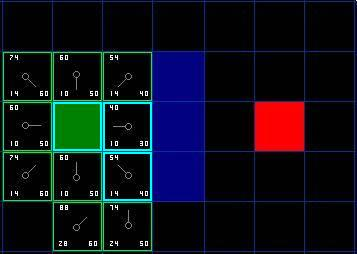
\includegraphics[width=.7\linewidth]{images/aStar2.jpg}
\caption{Upper-left number is F, Lower-left G and Lower-right H}
\label{fig:sub2}
\end{figure}

The A* algorithm is most commonly used in video games. The algorithm splits a known map into nodes (these can be any geometric shape, for example squares), and assigns a cost to each node. It also notes which nodes cannot be moves on, such as pits or walls. Based on this map, it determines the cost of movement from its position to some adjacent node(G), and estimates the cost of movement from that node to its final destination(H). It assigns this node with the value F which is the sum of G and H. It continues checking adjacent nodes with the same procedure, ocasionally changing the calculated path based on the F values of various nodes.\cite{astar}

In the early stages of robot automation, it was always assumed that the environment around the robot was known and the path was generated based on this. This was okay until the robot started to meet inconsistencies and obstacles in its path (This being discrepancies between the true state and the world state), the robot then either had to re-plan completely from scratch or alter the plan through trial-and-error. Computational wise, it would require too much power to re-plan from scratch (Even though this is the optimal choice) and most of the time trial-and-error does not yield an optimal outcome.


\clearpage
\begin{figure}[H]
        \centering
        \begin{subfigure}[H]{0.4\textwidth}
                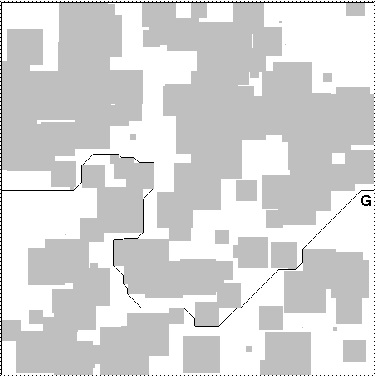
\includegraphics[width=\textwidth]{images/completemap.jpg}
                \caption{Complete Map}
                \label{fig:completemap}
        \end{subfigure}%
\quad
        \begin{subfigure}[H]{0.4\textwidth}
                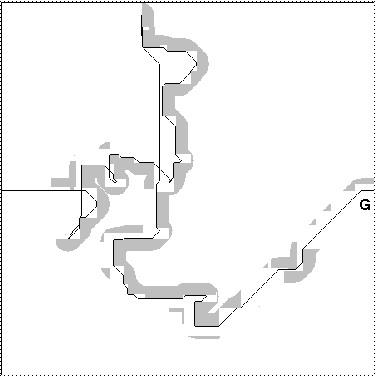
\includegraphics[width=\textwidth]{images/optimisticmap.jpg}
                \caption{Optimistic Map}
                \label{fig:optimisticmap}
        \end{subfigure}
        \caption{Mapping simulations with D*\cite{dstar}}\label{fig:animals}
\end{figure}

The D* algorithm creates an initial path based on assumed and known information, it then edits the path based on new information it receives whilst navigating the path. The final version of the edited plan is equivalent to replanning the whole thing from scratch, but avoids the limitations of the computation power.
Whenever an on-board sensor receives information about an obstacle, the algorithm can edit the path based on what possible routes there are available near by.
D* is fast at navigating large scale unknown environments because during its exploration its able to edit and repair its desired path and navigate towards its goal. It would require too much effort to re-plan everything from scratch every time it failed, especially for large scale environments.\cite{dstar}\cite{moredstar}

The figure(a) shows the map where the given robot knowns it's environment (The grey boxes) and can therefore easily determine the optimal path or the "Complete Map" in this case. Figure (b) on the other hand shows the "Optimistic Map", since before navigating on the planned path it assumes that there are no obstacles. Whenever the robot meets an obstacle during the optimistic map, it adjust it's course to continue towards its goal. On figure (b) it only displays the obstacles which the robot met during its journey navigation along the path.




Simple autonomous robots navigate by the use of infrared LEDs or by the use of photo-resistors and LEDS, by following lines drawn on a surface. Robots that use photo-resistors to follow a line are continuously looking for a change in brightness of the surface, if a the line-following robot is tracking a black line, then whenever the photo-resistor picks up the brightness from the surface that is not a black line, the path will change accordingly. A large number of photo-resistors can be used to increase the intelligence of an autonomous line-following robot, since the greater amount of LEDs can detect intersections between lines and different routes and be identified.\cite{linetrack}\\
Some autonomous robots and vehicles use multiples of different range sensors and other sensory equipment, to map and locate themselves in indoor and outdoor environments. The map that is generated can be used to keep track of static items in the environment such as structures and difference in terrain, but the map can also distinguish non-static items such as humans and other moving objects, from the static items. Since the maps are created by the vehicle itself whilst exploring, this technology can be used in places where there are no reference points, such as GPS\cite{rangesens}\cite{rangesensarc}. Robots and vehicles have been created using this technology to explore known and unknown environments. Because of advanced algorithms and hardware these autonomous devices are capable of performing some tasks more efficiently than humans, but are also able to perform them in places that are unsafe and hard to reach. %Add: for humans. ?

Autonomous robots also use these tools to work together. Using a shared map, the robots can keep track of one another and either perform tasks together or separately, depending on what is required from them.

\begin{figure}[H]
	\centering
	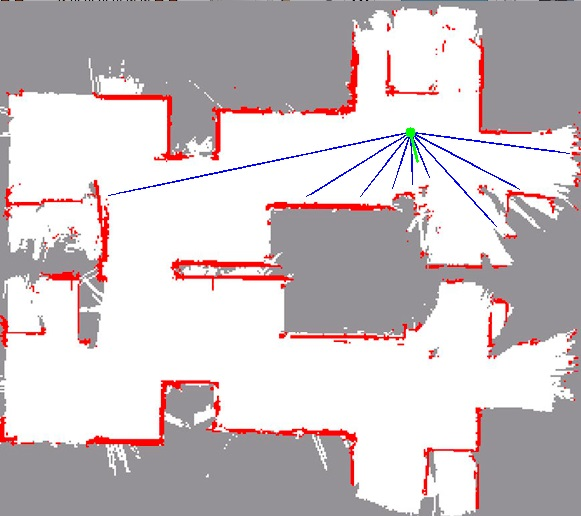
\includegraphics[scale=.7]{images/laserrangemap.jpg}
	\caption{Laser Range Map\cite{laserrangepic}}
	\label{fig:laserrangemap}
\end{figure}

Laser range finders and sonar arrays are used to navigate and determine the shortest possible path to a given destination. The sensory equipment is used to give the autonomous robot a sense of distance towards objects in an environment, giving it vital data regarding optimal travel directions and information on how to avoid obstacles\cite{lasersonar}.


%http://www.kuka-labs.com/en/service_robotics/mobile_robotics/autonomous_navigation/

%Advanced imagery stufferino
%http://ilab.usc.edu/publications/doc/Siagian_etal13icra.pdf

%Misc
%http://www.doc.ic.ac.uk/~nd/surprise_97/journal/vol4/jmd/
%http://www.doc.ic.ac.uk/~nd/surprise_97/journal/vol1/jmd/


